%!TEX root = paper.tex
\subsection{Solitary wave on a composite beach}
This is an laboratory experiment conducted at the Coastal Engineering Laboratory of the U.S. Army Corps of Engineers and it is described in \url{http://nctr.pmel.noaa.gov/benchmark/Solitary_wave/}, \url{http://chl.erdc.usace.army.mil/chl.aspx?p=s&a=Projects;36}. 
A linear solitary (better called single?) wave is propagating over a stepwise increasing bathymetry and it is reflected at a vertical wall on the right boundary. Different wave gauges measure the surface elevation and the runup on the vertical wall.

Three different cases A, B, C with different target wave heights $a_t$, actual (measured) wave heights $a$ and distances $L$ of gauge $G4$ to the first step in the bathymetry at gauge $G5$. Table \ref{tab:compositebeach_cases} displays the three different cases and belonging data. We only consider case A at the moment. Measured runup data can be found in table \ref{tab:compositebeach_runup}, but are not compared yet to the simulations.

\begin{table}[htbp]
\begin{tabular}{lllll}
\textbf{Case} & \textbf{target $a_t / d$} & \textbf{actual $a / d$} & \textbf{dist. G4 to G5 [m]} & \textbf{dist. G4 to Wall [m]}  \\
\toprule
A       &     0.05   & 0.039    &   2.4   &  10.59     \\
B       &     0.30   & 0.264    &   0.89  &   9.17     \\
C       &     0.70   & 0.696    &    0.64  &   8.83     \\
\bottomrule
\end{tabular}
\caption{Data of three different cases}
\label{tab:compositebeach_cases}
\end{table}


\begin{table}[htbp]
\begin{tabular}{lll}
\textbf{Case} & \textbf{Runup R [cm]} & \textbf{R / d} \\
\toprule
A       &        2.74   &  0.13 \\
B       &         45.72  &   2.10\\
C       &        27.43  &   1.26 \\
\bottomrule
\end{tabular}
\caption{Runup laboratory results of three different cases}
\label{tab:compositebeach_runup}
\end{table}


The initial condition is prescribed as a linear analytic solitary wave solution
\begin{align}
\xi(\bx,t)&=a \ \text{cosh}^{-2}(K(x-ct-x_0)), \\
u(\bx,t)&=c\frac{\xi(\bx,t)}{d},
\end{align}
with the initial amplitude $a$, propagation velocity $c=\csw$ on a stepwise reduced depth starting from $d=0.218 \, \text{m}$ with scale factor $K=\sqrt{\left(\frac{3a}{4d^3}\right)}$ and displacement $x_0=10.59$, s.t. the initial solitary wave has its maximum at gauge G4 with an entire domain length of $L=24 \, \text{m}$. The simulation time is $20$ seconds. 

We impose reflecting boundary conditions at the boundary in x-direction and periodic boundary conditions in y.direction. For the setup see figure \ref{fig:compositebeach_setup}. In both cases, the results are shifted by 271.5s to match the initial wave at gauge G4.

\begin{figure}[htbp]
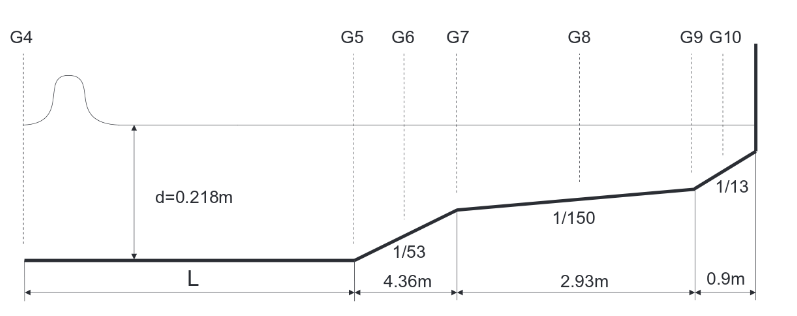
\includegraphics[width=\textwidth]{compositebeach_setup}
\caption{Setup of the testcase solitary wave on a composite beach}
\label{fig:compositebeach_setup}
\end{figure}

\subsubsection{Results of \nh\ model}
The linear SWE model results can be found in figure \eqref{fig:nh_compositebeach_ana_nh_Lhy}.

\begin{figure}[htbp]
\begin{minipage}{\textwidth}
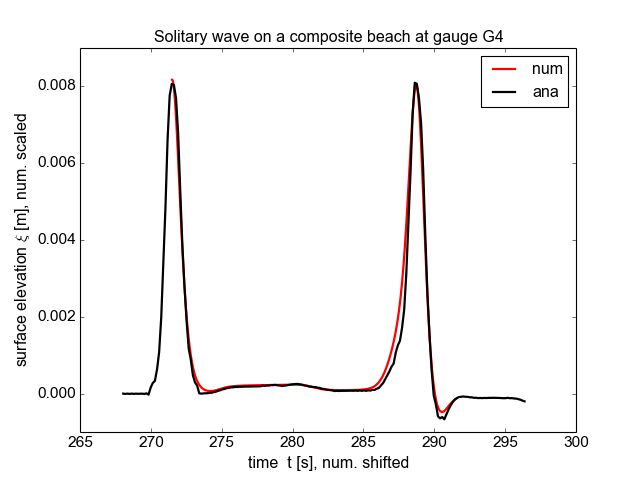
\includegraphics[width=0.48\textwidth]{compositebeach_ana_G4_nh_Lhy}
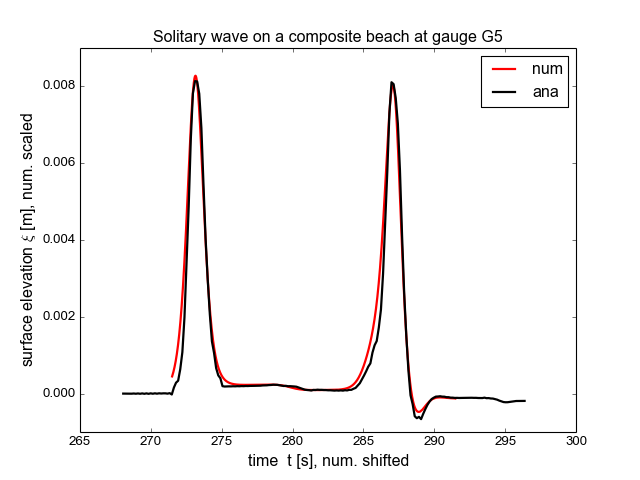
\includegraphics[width=0.48\textwidth]{compositebeach_ana_G5_nh_Lhy}
\end{minipage} \\
\begin{minipage}{\textwidth}
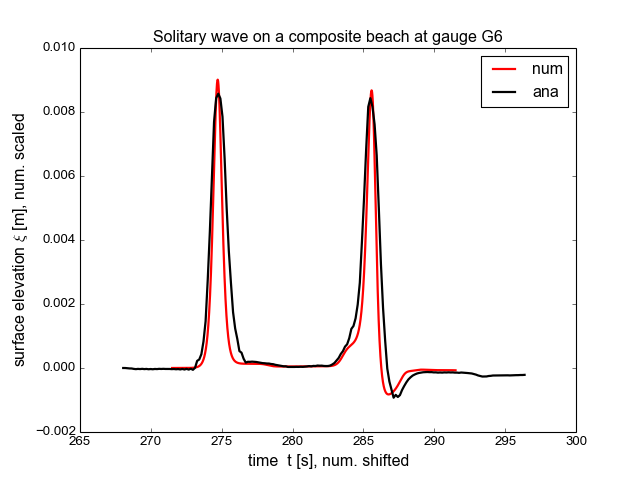
\includegraphics[width=0.48\textwidth]{compositebeach_ana_G6_nh_Lhy}
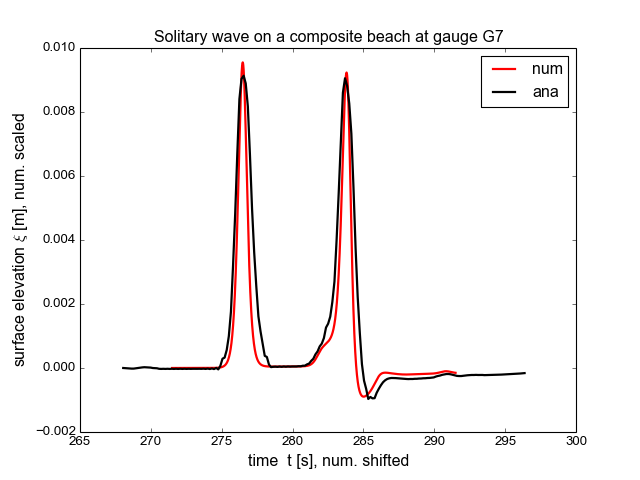
\includegraphics[width=0.48\textwidth]{compositebeach_ana_G7_nh_Lhy}
\end{minipage} \\
\begin{minipage}{\textwidth}
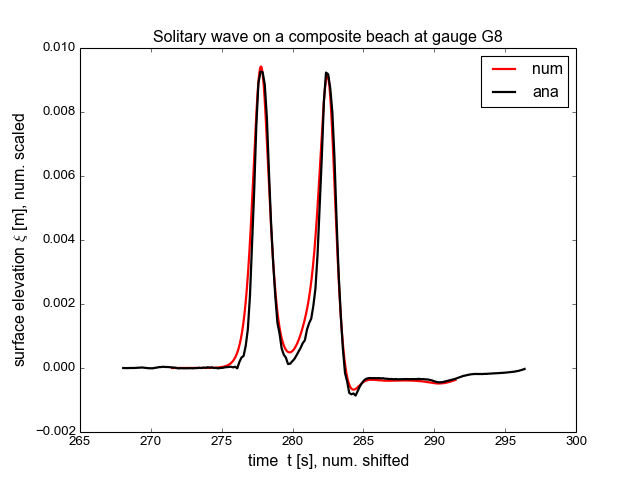
\includegraphics[width=0.48\textwidth]{compositebeach_ana_G8_nh_Lhy}
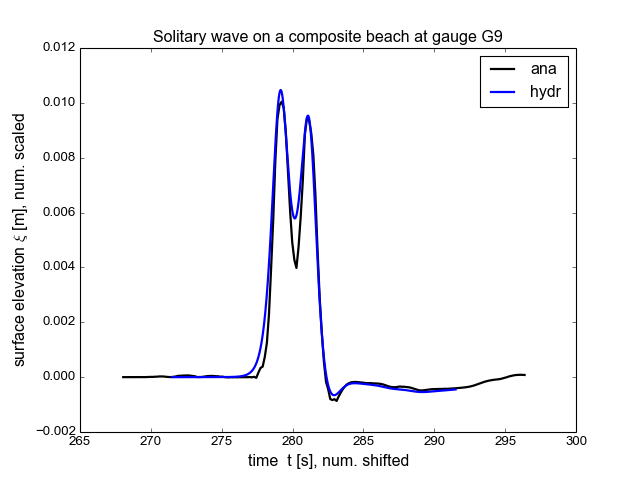
\includegraphics[width=0.48\textwidth]{compositebeach_ana_G9_nh_Lhy}
\end{minipage} \\
\begin{minipage}{\textwidth}
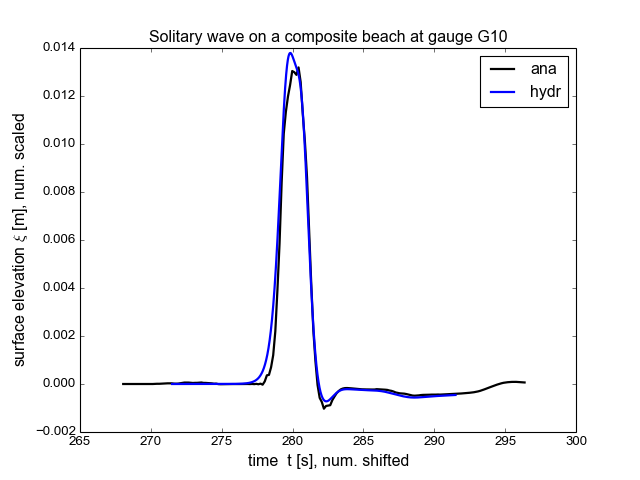
\includegraphics[width=0.48\textwidth]{compositebeach_ana_G10_nh_Lhy}
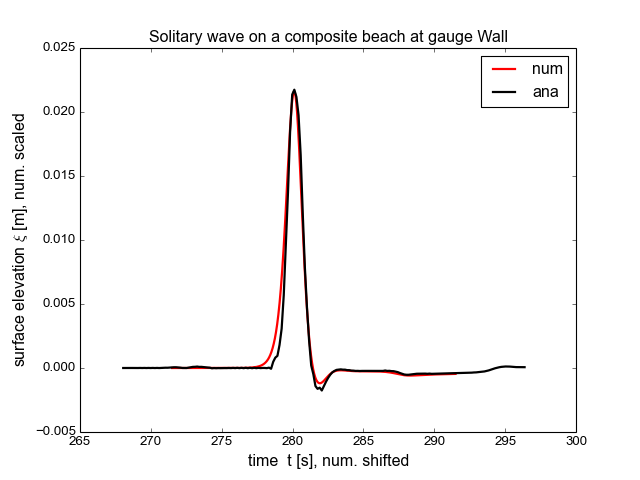
\includegraphics[width=0.48\textwidth]{compositebeach_ana_Wall_nh_Lhy}
\end{minipage}
\caption{Comparison of the analytical (black) sea surface height of the
solitary wave with the simulation results of the \nh\ model in its version of linear shallow water equations (red)}
\label{fig:nh_compositebeach_ana_nh_Lhy}
\end{figure}
